\documentclass[aspectratio=43]{beamer}
\usepackage[english]{babel}
\usepackage[utf8]{inputenc}
\usepackage{xcolor}
\usepackage{amsthm}
\usepackage{mathtools}
\usepackage{physics}
\usepackage{calligra}
\usepackage{csquotes}
\usepackage{tensor}
\usepackage[thicklines]{cancel}
\usepackage{tcolorbox}
\usepackage{pstricks}
\usepackage[backend=biber, bibstyle=nature, sorting=nty, citestyle=numeric-comp]{biblatex} %Custom bibliography
    \addbibresource{bib.bib} %Load references


\DeclareMathAlphabet{\mathcalligra}{T1}{calligra}{m}{n}
\DeclareFontShape{T1}{calligra}{m}{n}{<->s*[2.2]callig15}{}
\newcommand{\scriptr}{\mathcalligra{r}\,}
\newcommand{\boldscriptr}{\pmb{\mathcalligra{r}}\,}
\def\rc{\scriptr}
\def\brc{\boldscriptr}
\def\hrc{\hat\brc}
\newcommand{\ie}{\emph{i.e.}} %id est
\newcommand{\eg}{\emph{e.g.}} %exempli gratia
\newcommand{\rtd}[1]{\ensuremath{\left\lfloor #1 \right\rfloor}}
\newcommand{\dirac}[1]{\ensuremath{\delta \left( #1 \right)}}
\newcommand{\diract}[1]{\ensuremath{\delta^3 \left( #1 \right)}}
\newcommand{\e}{\ensuremath{\epsilon_0}}
\newcommand{\m}{\ensuremath{\mu_0}}
\newcommand{\V}{\ensuremath{\mathcal{V}}}
\newcommand{\prnt}[1]{\ensuremath{\left(#1\right)}} %parentheses
\newcommand{\colch}[1]{\ensuremath{\left[#1\right]}} %square brackets
\newcommand{\chave}[1]{\ensuremath{\left\{#1\right\}}}  %curly brackets

\useoutertheme{infolines}
\useinnertheme{rectangles}
\usefonttheme{professionalfonts}


\definecolor{orange}{rgb}{0.95, 0.5, 0.4}
\definecolor{gray}{rgb}{0.2, 0.2, 0.2}
\definecolor{yellow}{rgb}{0.95, 0.75, 0.3}
\definecolor{lightorange}{rgb}{0.95, 0.6, 0.35}

\renewcommand{\CancelColor}{\color{orange}}

\makeatletter
\newcommand{\mybox}[1]{%
  \setbox0=\hbox{#1}%
  \setlength{\@tempdima}{\dimexpr\wd0+13pt}%
  \begin{tcolorbox}[colback=orange,colframe=orange,boxrule=0.5pt,arc=4pt,
      left=6pt,right=6pt,top=6pt,bottom=6pt,boxsep=0pt,width=\@tempdima]
    \textcolor{white}{#1}
  \end{tcolorbox}
}
\makeatother

\usecolortheme[named=orange]{structure}
\usecolortheme{sidebartab}
\usecolortheme{orchid}
\usecolortheme{whale}
\setbeamercolor{alerted text}{fg=yellow}
\setbeamercolor{block title alerted}{bg=alerted text.fg!90!black}
\setbeamercolor{block title example}{bg=lightorange!60!black}
\setbeamercolor{background canvas}{bg=gray}
\setbeamercolor{normal text}{bg=gray,fg=white}

\setbeamertemplate{footline}
        {
      \leavevmode%
      \hbox{%
      \begin{beamercolorbox}[wd=.333333\paperwidth,ht=2.25ex,dp=1ex,center]{author in head/foot}%
        \usebeamerfont{author in head/foot}\insertshortauthor~~(\insertshortinstitute)
      \end{beamercolorbox}%
      \begin{beamercolorbox}[wd=.333333\paperwidth,ht=2.25ex,dp=1ex,center]{title in head/foot}%
        \usebeamerfont{title in head/foot}\insertshorttitle
      \end{beamercolorbox}%
      \begin{beamercolorbox}[wd=.333333\paperwidth,ht=2.25ex,dp=1ex,center]{date in head/foot}%
        \usebeamerfont{date in head/foot}\insertshortdate{}%\hspace*{2em}

    %#turning the next line into a comment, erases the frame numbers
        %\insertframenumber{} / \inserttotalframenumber\hspace*{2ex} 

      \end{beamercolorbox}}%
      \vskip0pt%
    }


\setbeamertemplate{blocks}[rectangle]
\setbeamercovered{dynamic}

\setbeamertemplate{section page}
{
	\begin{centering}
		\begin{beamercolorbox}[sep=27pt,center]{part title}
			\usebeamerfont{section title}\insertsection\par
			\usebeamerfont{subsection title}\insertsubsection\par
		\end{beamercolorbox}
	\end{centering}
}

%\setbeamertemplate{subsection page}
%{
%	\begin{centering}
%		\begin{beamercolorbox}[sep=12pt,center]{part title}
%			\usebeamerfont{subsection title}\insertsubsection\par
%		\end{beamercolorbox}
%	\end{centering}
%}

\newcommand{\hlight}[1]{\colorbox{violet!50}{#1}}
\newcommand{\hlighta}[1]{\colorbox{red!50}{#1}}
\title{Da li ste bezbedni na Internetu?}
\author[Ajvaz, Jovanović, Milićević, Nikčević]{Nevena Ajvaz, Natalija Jovanović, Marija Milićević, Tijana Nikčević}
\institute[MatF]{
    Matematički fakultet,%
    \\%
    Univerzitet u Beogradu%
} 
\date{15. maj 2019.}

\graphicspath{ {./images/} }

\expandafter\def\expandafter\insertshorttitle\expandafter{%
  \insertshorttitle\hfill%
  \insertframenumber\,/\,\inserttotalframenumber}

\begin{document}
    
    \frame{\titlepage}    
    \begin{frame}{Sadržaj}
        \tableofcontents
    \end{frame}
    
    \section{Sajber kriminal i napadi}

\begin{frame}{Pojam sajber kriminala}
        
        %\noindent\begin{minipage}{0.6\linewidth}
        \begin{itemize}
        	\item \textit{def.} Visokotehnološki ili sajber kriminal (eng. cyber crime) predstavlja moderni vid kriminala, tj. putem mreže kako bi se izvele zlonamerne aktivnosti
            
			\item cilj je krađa osetljivih podataka neke firme, lične informacije ili profit
            
        \end{itemize}
    \end{frame}
    
    
   \begin{frame}{Zakon u Srbiji}
    \begin{itemize}
    \item globalni indeks sajber bezbednosti (eng. GCI) - pouzdan izvor koji meri posvećenost država bezbednosti na Internetu 
    \item Srbija je zemlja sa niskom stopom posvećenosti suzbijanju sajber kriminala
    \end{itemize}
	\begin{minipage}{0.3\textwidth}
        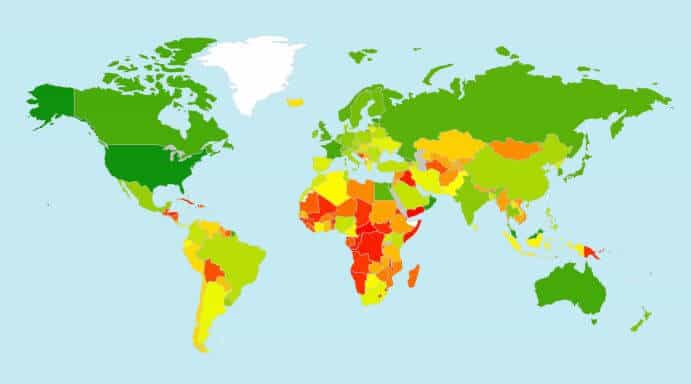
\includegraphics[scale = 0.25]{itu_worldmap.jpg}
        \end{minipage}
        \begin{minipage}{0.6\textwidth}\raggedleft
        Tamnozelena-najviše posvećen\\
        crvena-najmaje posvećen\\
        \end{minipage}
        %\noindent
    \end{frame}
    
    \begin{frame}{Sajber napadi i vrste}
    \begin{itemize}
	\item \textit{def.} Sajber napad - napad od računara do računara koji povređuje poverljivost, integritet i informacije koje se nalaze na napadnutom računaru  
	\item sa porastom popularnosti Interneta porasla je i stopa kriminala na njemu
	\item najčešće vrste napada
	\begin{itemize}
	\item Fišing (eng. phishing)
	\item SQL injekcija
	\item DoS napadi
\end{itemize}	  
    \end{itemize}
    \end{frame}
    
    %\frame{\sectionpage}
    
    \begin{frame}{Fišing (eng. \textit{phishing})}
        
        \noindent\begin{minipage}{0.55\linewidth}
            \begin{itemize}
                \item lažno predstavljanje pomoću elektronske pošte ili zlonamernih veb sajtova kako bi se prikupili lični podaci
                \item termin phishing: phreaks + fishing
                \item mejlovi obaveštavaju primaoce da je njihov nalog kompromitovan
                \item ciljano orijentisan fising \\(eng. spear phishing)
            \end{itemize}
        \end{minipage}
        \hfill
        \begin{minipage}[t]{0.4\linewidth}
            \centering
            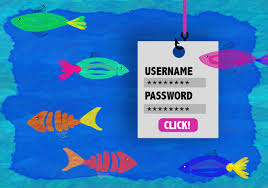
\includegraphics[scale = 0.3]{images/phishing1.jpeg}
            \vspace{0.5cm}
            \includegraphics[scale = 0.3]{images/spear_phishing_transparent.png}
        \end{minipage}
        %\includegraphics[scale = 0.3]{spear_phishing_transparent.png}
    \end{frame}
    
    \begin{frame}{Fišing (eng. \textit{phishing})}
        \begin{minipage}{0.6\textwidth}
        \begin{itemize}
                \item fišing se pojavio negde oko 1995. (AOL)
                \item 2000ih godina su napadi prešli na platne sisteme (E-Gold, eBay i PayPal)
            \end{itemize}
        \end{minipage}
        \begin{minipage}[t]{0.3\linewidth}
            \centering
            
\includegraphics[scale = 0.045]{images/aol_logo.jpg}
            \hspace{0.1cm}
            
\includegraphics[scale = 0.05]{images/PayPal_eBay.jpg}
        \end{minipage}
        
        \begin{minipage}{\textwidth}
            \centering
            \vspace{0.3cm}
            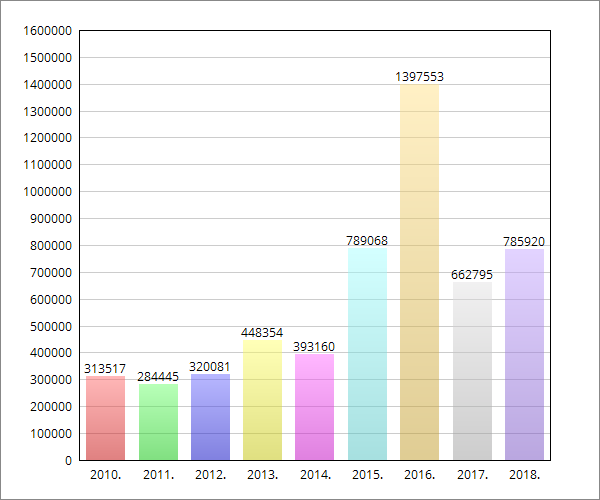
\includegraphics[width=0.7\textwidth, height = 5cm]{images/phishing.png}
        \end{minipage}
        \begin{minipage}{\textwidth}
            \centering
            \textit{broj sajtova za fišing koje je APWG otkrio tokom godina}
        \end{minipage}
    \end{frame}

\begin{frame}{SQL injekcija}
        
        %\noindent\begin{minipage}{0.6\linewidth}
            \begin{itemize}
                \item umetanje dela ili celog SQL upita obično preko polja za unos na veb stranici
                \item načini upotrebe SQL injekcije:
                		\begin{itemize}
                		\item \texttt{1=1} je uvek istinito
                		        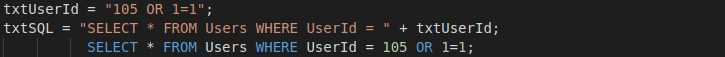
\includegraphics[width=\linewidth]{sql1.png}
                		\item \texttt{"}\texttt{"}=\texttt{"}\texttt{"} je uvek istinito
                		        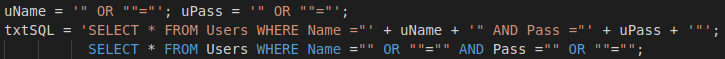
\includegraphics[width=\linewidth]{sql2.png}                		        
                		\item grupa SQL upita razdvojenih ; simbolom
                		        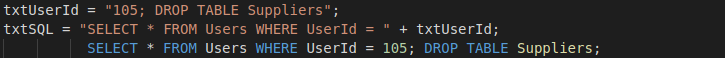
\includegraphics[width=\linewidth]{sql3.png}
                		\end{itemize}
                	\item zaštita od ovakvih napada je moguća korišćenjem SQL parametara
            \end{itemize}
    \end{frame}


\begin{frame}{DoS napadi (eng. \textit{Denial-of-Service})}

	\begin{itemize}

		\item napadač - ometa usluge servera i čini ga nedostupnim svojim korisnicima
		\item asimetričan napad - jedna osoba može dosta da naškodi velikoj organizaciji
		\item cilj - remećenje sposobnosti servera, a ne krađa informacija
		\item dodatni tip DDoS (eng. \textit{Distributed Denial-of-Service}) - meta je napadnuta sa više lokacija odjednom
		\item zaštita - razviti plan odgovora na napad, osigurati mrežnu infrastrukturu, održavati jaku arhitekturu mreže, razumeti znakove upozorenja

	\end{itemize}

\end{frame}


\begin{frame}{Primeri napada}

	\noindent\begin{minipage}{0.55\linewidth}
	%\vspace{1cm}
    \begin{itemize}

    \item samostalni napadi
    	\begin{itemize}
    		\item Dženson Džejms Ančeta
    		\item PharmaMaster
    	\end{itemize}
    
    \item napadi na države
    	\begin{itemize}
    		\item Gruzija
    		\item SAD i Južna Koreja
    	\end{itemize}
    	
    \item napadi na kompanije
    	\begin{itemize}
    		\item Yahoo!
    		\item eBay
    	\end{itemize}
    \end{itemize}
        \end{minipage}
        
        \hfill
        \begin{minipage}[t]{0.5\linewidth}
            \centering
	        \vspace{-4cm}
            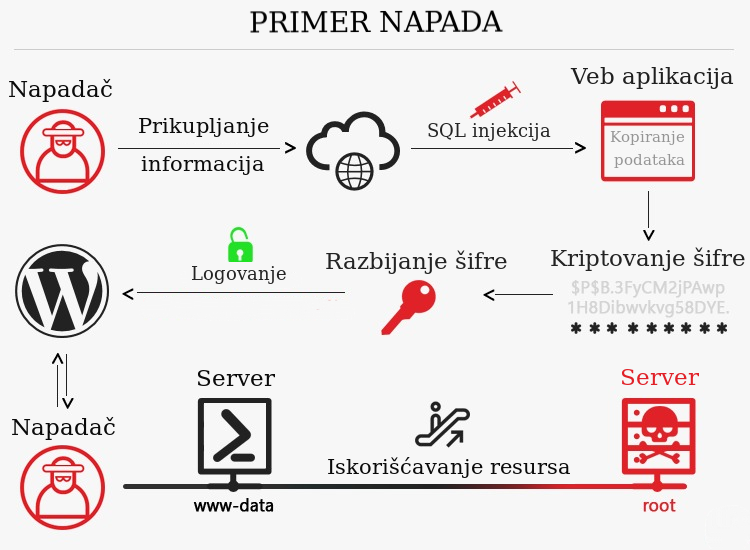
\includegraphics[scale = 0.2]{images/napad.png}
        \end{minipage}
    
    \end{frame}
    

\begin{frame}{Sajber kriminal}

	\begin{itemize}
		
		\item zlonameran k\^{o}d (eng. \textit{malware}) - glavno sredstvo za trgovinu informacijama i infiltriranje u sisteme
		\item napadači - jako pažljivi i prikrivaju svoje tragove
		\item botnet-ovi - podstiču rast sajber napada i dozvoljavaju napadaču da kontroliše neki sistem širom Interneta
		
	\end{itemize}

\end{frame}
    
    \section{Glasanje putem Interneta}

\begin{frame}{Glasanje putem Interneta}
        \begin{minipage}{0.6\textwidth}
            \begin{itemize}
                \item problemi sa glasovima države Florida, 
                \\predsednički izbori SAD, \\2000. godina
                \item akcije za poboljšanje pouzdanosti glasačkih sistema
                \item Estonija - 2005. godina
                \item Norveška - 2011. i 2013. godina
            \end{itemize}
        \end{minipage}
        \begin{minipage}{0.3\linewidth}
            \centering
            
            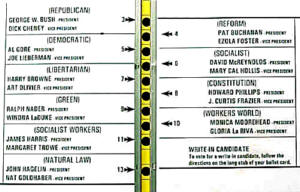
\includegraphics[scale = 1]{images/election.jpg}
        \end{minipage}
        
        \begin{itemize}
            \item danas je glasanje putem Interneta omogućeno u 14 zemalja \\(Kanada, Francuska, Švajcarska...)
        \end{itemize}
    \end{frame}
    
    
    \begin{frame}{Benefiti glasanja putem Interneta}
    		\begin{itemize}
    			\item daje ljudima priliku da glasaju iz svojh domova
			\item brže prebrojavanje glasova
			\item nema dvosmislenosti
			\item manji trošak
            \item eliminisanje rizika da neko manipuliše glasačkom kutijom
            \item obrazac za glasanje sa različitim ograničenjima
			\item veb forma dizajnirana više strana 
    		\end{itemize}
    \end{frame}
    
    
    \begin{frame}{Rizici glasanja putem Interneta}
    	\begin{itemize}
			\item daje prednost onima koji su u finansijski boljoj situaciji
			\item isti sistem vrši autentifikaciju glasača i beleži glasački listić
			\item povećava mogućnost za kupovinu i prodaju glasova.
			\item veb lokacija koja održava izbore očigledna je meta DDoS napada
			\item \textit{backdoor} Trojanac (eng. {\em backdoor Trojan}) koji vreba na računaru glasača
			\item napadač može da prevari korisnika da misli da je povezan sa serverom za glasanje kada je u stvari povezan sa lažnim serverom za glasanje koji je kontrolisan od strane napadača	
		\end{itemize}
    \end{frame}
    
    \section{Literatura}
    \nocite{knjiga}
    	\nocite{sql_injection}
    	\nocite{gci}
    \begin{frame}{Literatura}
		\printbibliography
	\end{frame}

    \section{}
    \begin{frame}{}
        \centering
            \Huge\bfseries
        \textcolor{orange}{Hvala na pažnji!\\ Pitanja?}
    \end{frame}
\end{document}
